\section{Introduction}
This report is based on a project made during the 2022 spring course of \href{https://learnit.itu.dk/local/coursebase/view.php?ciid=909}{DevOps, Software Evolution and Software Maintenance, MSc} with the following  \href{https://github.com/itu-devops/lecture_notes/tree/e44664f50c8b0ffb30a77a29e305df3f6750d5d4}{Course material}. 

The project's focus was on making software that can evolve, scale and be maintained. An old application copying the social media platform Twitter, that had not been touched for years was provided to us. From this we were to create our scalable, maintainable, and automatically deployed version, which we named MiniTwit, see \autoref{fig:Minitwit_public}.

\begin{figure}[!ht]
    \centering
    \captionsetup{justification=centering,margin=1cm}
    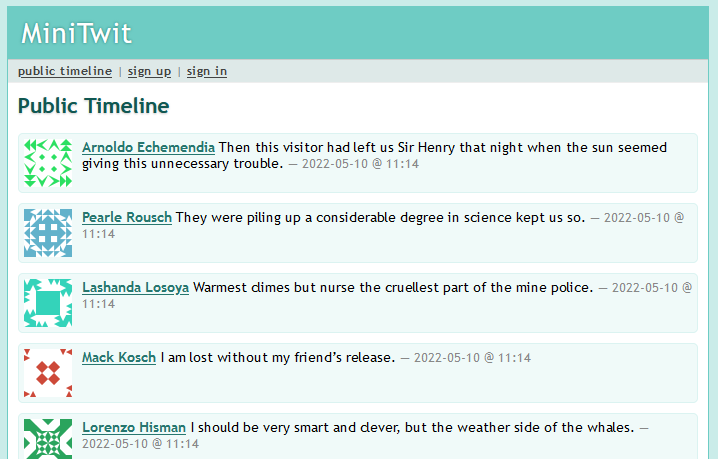
\includegraphics[width=80mm]{images/introduction/minitwitFrontPage.png}
    \caption{Front page of MiniTwit as a public user (Source: Own image)}
    \label{fig:Minitwit_public}
\end{figure}

To generate traffic to the site, the professors have created a simulator see \autoref{fig:Simulator} which stress test the system, and simulate a scenario/environment, where downtime is punished. 

\begin{figure}[h!]
  \centering
  \begin{subfigure}[b]{0.45\linewidth}
    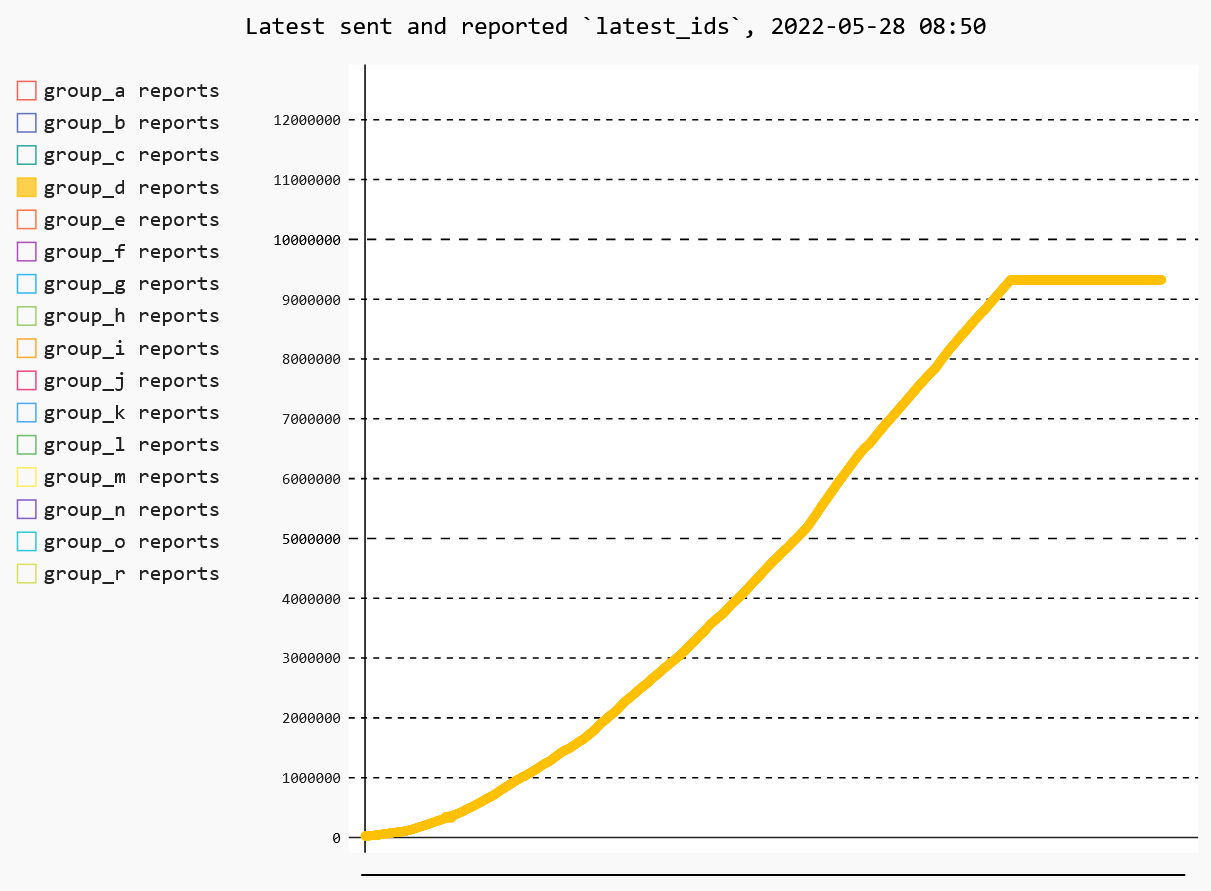
\includegraphics[width=\linewidth]{images/introduction/latest_group_d.png}
    \caption{The flow of requests from the simulator.}
  \end{subfigure}
  \begin{subfigure}[b]{0.45\linewidth}
    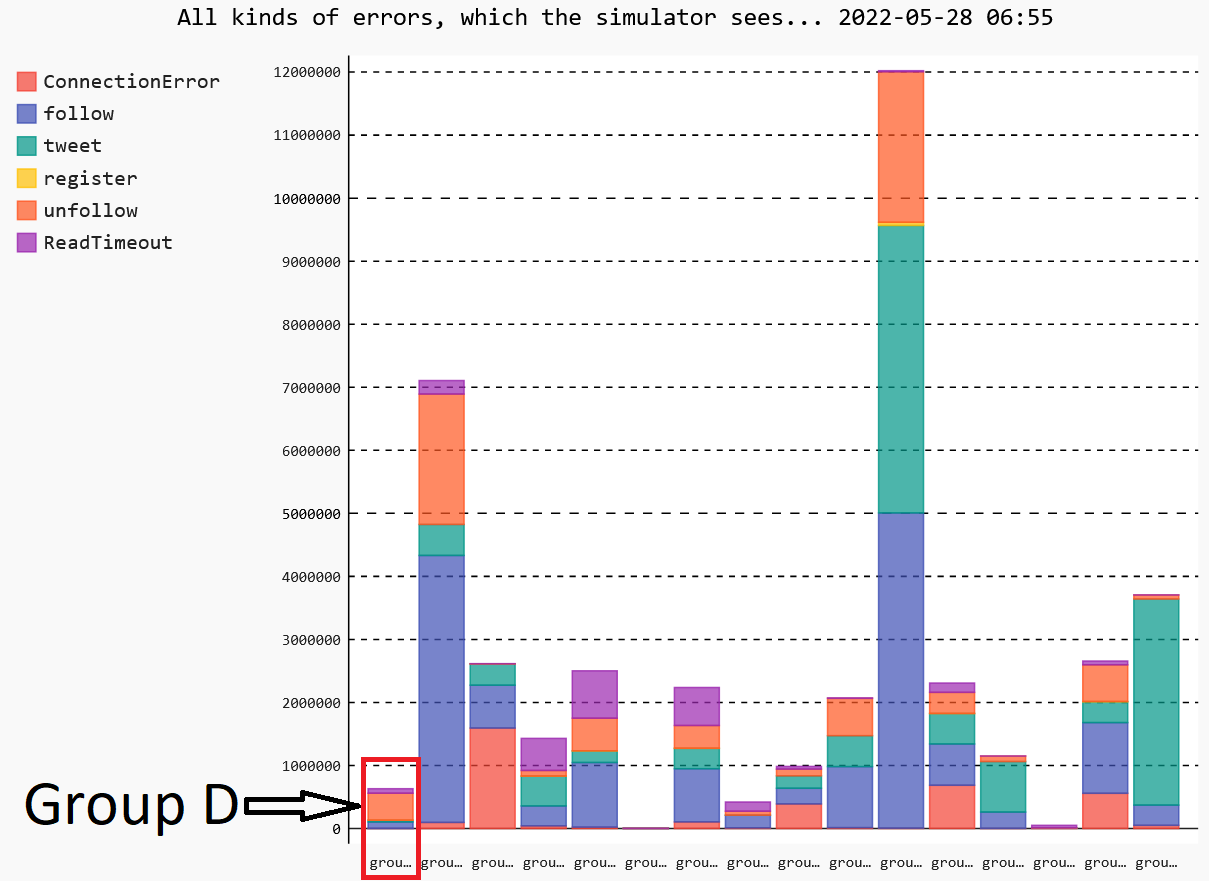
\includegraphics[width=\linewidth]{images/introduction/errors_group_d.png}
    \caption{Errors seen from the simulator}
  \end{subfigure}
  \caption{Feedback loop from the simulator to the groups (Source: \href{http://164.92.246.227/status.html}{Simulator})}
  \label{fig:Simulator}
\end{figure}

To enable discussion of the system from different views the following roles have been defined.

\begin{itemize}
    \item \textbf{Product owners}: The group
    \item \textbf{Stakeholder}: The professors
    \item \textbf{Customers}: The simulator / users of the service.
\end{itemize}

%\todo{Mention that all links starting with \#xxx is a reference to the Minitwit or the ServerDeployment repository.}
  